\documentclass[tikz, a4paper]{nmd/hw}
\begin{document}
\classtemplate{Nathan PS}{Warwick School}{\hfill}

For lecture notes, references, and links to SnapPy, SageMath, etc see:
\\
\url{http://dunfield.info/warwick2017}

%\textbf{The math behind SnapPy.}  See the excellent paper: J. Weeks, \emph{Computation of Hyperbolic Structures in Knot Theory}, \href{http://arxiv.org/abs/math/0309407}{arXiv:0309407}

\begin{problems}
\item A \3-manifold is \emph{irreducible} if every smoothly embedded
  2-sphere bounds a 3-ball.  For example, a basic topological fact is
  that $\R^3$ and $S^3$ are irreducible.
  \begin{enumerate}
    \item Show the only closed orientable 3-manifold which is prime
      but not irreducible is $S^2 \times S^1$.
    \item Prove that if $\Mtil \to M$ is a covering map and $\Mtil$ is
      irreducible then so is $M$.

    \item Use (b) to show that $T^3$ and all the lens
      spaces $L(p,q)$ are irreducible.
  \end{enumerate}

\item For an orientable closed surface $S$ with some fixed Riemannian
  metric, consider the circle bundle
  $UT(S) = \setdef{v \in T_*S}{\norm{v} = 1}$ of unit-length tangent
  vectors.  (The topology of $UT(S)$ does not depend on the metric.)
  Show that $UT(S)$ admits a Riemannian metric modelled on one of the
  eight Thurston geometries.  Hint: Which geometry to pick depends on $S$!
  
\item Prove that $T^3 \# T^3$ cannot be given a geometric structure
  modelled on one of the eight Thurston geometries.

\item Another purely topological corollary of the Geometrization Theorem is:

  \emph{Suppose $M$ is a closed \3-manifold.  If $M$ is not $S^3$ then it
    has a nontrivial finite cover $\Mtil \to M$.  Equivalently, the
    group $\pi_1(M)$ has a nontrivial subgroup of finite-index.}

  In fact, it turns out that $\pi_1(M)$ is residually finite.  Prove
  the corollary when $M$ is hyperbolic.  Hint: Note that $\pi_1(M)$ is
  a subgroup of $\PSL{2}{\C}$ and Google ``Malcev's theorem linear
  groups''.  What kind of issues would arise when tackling the general
  case?

\item Suppose $M$ is a closed hyperbolic $n$-manifold.
  \begin{enumerate}
  \item Prove that every $\gamma \neq 1$ in $\pi_1(M)$ is homotopic to
    a unique closed geodesic.
    
  \item Prove that for every $L \geq 0$ there are finitely many closed
    geodesics of length at most $L$.

  \item Prove that the isometry group of $M$ is finite.
  \end{enumerate}

\item The remaining problems all involve practical computation with
  hyperbolic structures, so the first step is to download and install
  \textbf{SnapPy 2.5.4} from \url{http://snappy.computop.org}

\item \begin{enumerate}
  \item Load the manifold $v1234$ and name it $V$.  
  \item Use the browser to find the volume, Dirichlet domain, and
    symmetry group of $V$.
  \item Like any manifold in SnapPy, the object $V$ is really a
    particular \emph{triangulation} of this hyperbolic manifold.
    Back at the command line, determine the number of tetrahedra
    in the triangulation $V$.  Hint: Use tab completion by
    typing \texttt{V.<tab-key>}.  
  \item The manifold $V$ has one cusp.  Back the browser, do Dehn
    filling along the meridian curve.  What closed manifold do you get?  
  \end{enumerate}
  
  \item 
    \begin{minipage}[t]{8.5cm}
      \begin{enumerate}
      \item Use SnapPy to find the name in the Rolfsen table for the link shown at
        right. 
      \item Is the projection at right the same as the one that's stored
        in SnapPy?  
      \end{enumerate}
    \end{minipage}\quad
    \begin{minipage}[t]{12cm}
      \hbox{}
      \vspace{-1cm}
      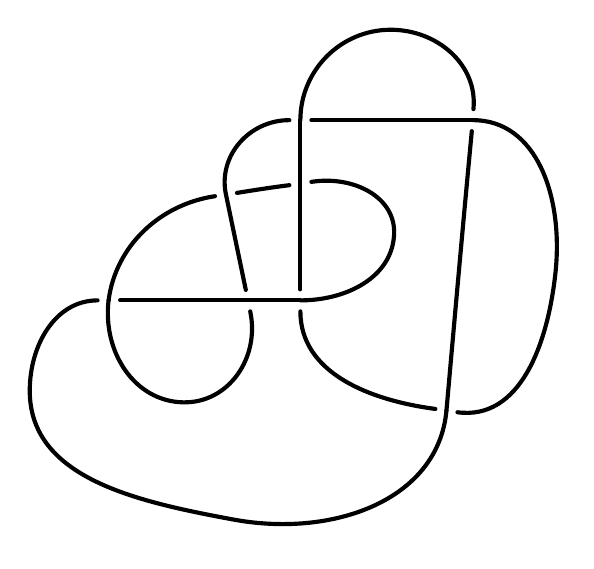
\begin{tikzpicture}[scale=0.7, line width=1.5, line cap=round, line join=round]
        \begin{scope}[color=black]
          \draw (7.49, 2.49) .. controls (6.28, 2.65) and (5.04, 3.15) .. (5.04, 4.26);
          \draw (5.04, 4.66) .. controls (5.04, 5.30) and (5.04, 5.94) .. (5.04, 6.58);
          \draw (5.04, 6.58) .. controls (5.04, 6.97) and (5.04, 7.35) .. (5.04, 7.73);
          \draw (5.04, 7.73) .. controls (5.04, 8.63) and (5.77, 9.37) .. 
          (6.68, 9.37) .. controls (7.53, 9.37) and (8.26, 8.73) .. (8.18, 7.93);
          \draw (8.15, 7.53) .. controls (7.99, 5.84) and (7.84, 4.15) .. (7.69, 2.46);
          \draw (7.69, 2.46) .. controls (7.54, 0.83) and (5.62, 0.14) .. 
          (3.79, 0.49) .. controls (2.08, 0.81) and (0.13, 1.23) .. 
          (0.13, 2.82) .. controls (0.13, 3.66) and (0.60, 4.46) .. (1.36, 4.46);
          \draw (1.77, 4.46) .. controls (2.54, 4.46) and (3.31, 4.46) .. (4.09, 4.46);
          \draw (4.09, 4.46) .. controls (4.41, 4.46) and (4.72, 4.46) .. (5.04, 4.46);
          \draw (5.04, 4.46) .. controls (5.88, 4.46) and (6.70, 4.88) .. 
          (6.74, 5.65) .. controls (6.78, 6.33) and (6.01, 6.73) .. (5.24, 6.61);
          \draw (4.84, 6.55) .. controls (4.52, 6.51) and (4.20, 6.46) .. (3.89, 6.41);
          \draw (3.49, 6.35) .. controls (2.49, 6.20) and (1.69, 5.45) .. (1.56, 4.46);
          \draw (1.56, 4.46) .. controls (1.45, 3.52) and (2.03, 2.63) .. 
          (2.91, 2.61) .. controls (3.73, 2.59) and (4.31, 3.41) .. (4.13, 4.26);
          \draw (4.05, 4.65) .. controls (3.93, 5.23) and (3.81, 5.80) .. (3.69, 6.38);
          \draw (3.69, 6.38) .. controls (3.54, 7.08) and (4.11, 7.73) .. (4.84, 7.73);
          \draw (5.24, 7.73) .. controls (6.22, 7.73) and (7.19, 7.73) .. (8.17, 7.73);
          \draw (8.17, 7.73) .. controls (9.33, 7.73) and (9.81, 6.34) .. 
          (9.67, 4.98) .. controls (9.53, 3.65) and (9.02, 2.28) .. (7.89, 2.43);
        \end{scope}
      \end{tikzpicture}
  \end{minipage}

\item In my lecture, I mostly focused on manifolds with cusps, but
  SnapPy also works with closed manifolds.  In particular, it comes
  with the Hodgson-Weeks census of small-volume closed hyperbolic
  3-manifolds, which is called \texttt{OrientableClosedCensus}.

  \begin{enumerate}
    \item Use the ``?'' operator to find out more about
      \texttt{OrientableClosedCensus}; in particular, how many
      manifolds are in it?  

      Also, interrogate the orientable \emph{cusped} census to get
      ideas on how to select various types of manifolds for the later
      parts of this question.
      
    \item Closed manifold in SnapPy are represented as Dehn fillings
      on cusped manifolds.  You can do Dehn filling in the browser,
      via the \texttt{dehn\_fill} method, or as part of the
      specification that you given to \texttt{Manifold}.  For example,
      typing \texttt{A = Manifold(`4\_1(1,2)')} gives the closed
      3-manifold which is $\frac{1}{2}$-Dehn surgery on the figure 8
      knot.  Use the method \texttt{is\_isometric\_to} to show that
      $A$ is the sixth manifold the \texttt{OrientableClosedCensus}.
      Warning: In Python, lists are numbered starting from 0
      rather than 1.

    \item Find the unique manifold $M$ in the original
      \texttt{OrientableClosedCensus} whose volume is between $3.0$
      and $3.1$ and whose first homology is
      $\Z/3\Z \oplus \Z/3\Z \oplus \Z/3\Z$.

    \item Find a description of $M$ as Dehn surgery on a 3-component
      link in $S^3$.  Hint: Unfill the cusp in the default description
      of $M$ and then drill out the shortest geodesic twice.  

  \end{enumerate}



\end{problems}


\end{document}